% =====================================================================
%  Capítulo 4 — Implementação
% =====================================================================
\chapter{Implementação}
\label{cap:implementacao}
\rubricaFuncionalidade

\begin{orientacao}
Este é o capítulo que responde \enquote{o protótipo funciona?}, que vale
30\,\% da nota. Ele descreve o que foi construído, com detalhe
suficiente para que outra equipe consiga reproduzir. O critério prático:
se alguém com o repositório e este capítulo na mão não conseguir montar
e rodar o sistema, falta coisa aqui.
\end{orientacao}

Este capítulo descreve \textbf{dois \emph{firmwares}}. O primeiro é o
nó da AP1, \texttt{esp32\_dht22.ino}, que lê, filtra e alarma, mas não
publica. Em relação à primeira versão dele, três coisas mudaram e são
detalhadas aqui: o intervalo entre
leituras e os limiares de faixa deixaram de ser constantes de
compilação e passaram a ser \textbf{parâmetros gravados em memória
não-volátil} (biblioteca \texttt{Preferences}); o \textbf{alarme local}
(buzzer ativo + LED) foi integrado ao \emph{firmware}; e, enquanto a
leitura está fora da faixa, o nó passa a acordar em um
\textbf{intervalo mais curto} do que o de rotina. O custo de cada uma
dessas mudanças em tempo acordado e em energia é declarado nas seções
correspondentes.

O segundo é o \emph{firmware} de comunicação, construído na AP2 à
parte, sobre o nó MQTT do Lab~03 (Seção~\ref{sec:firmware-com}, branch
\texttt{lab3}): o nó entra no WiFi, acerta o relógio por NTP, conecta ao
\emph{broker} por TLS deixando um testamento \texttt{offline}, publica
\texttt{online} retido, assina o próprio tópico de configuração e
publica cada leitura no contrato de dados da
Seção~\ref{sec:contrato-dados}, com QoS~1. Em relação ao sketch-base, a
equipe trocou o sensor do exemplo (um MPU6050 em I\textsuperscript{2}C)
pelo DHT22 no \texttt{GPIO4}, o mesmo pino da AP1, com a biblioteca
DHTesp; definiu a equipe e o nó (\texttt{eq01}, \texttt{no02}); e
passou o monitor serial de 9600 para \SI{115200}{\baud}, a velocidade que
o roteiro do Lab~03 manda usar.
\textbf{Esse \emph{firmware} não tem} a leitura filtrada da AP1 (mediana
de 5 amostras e EMA), o alarme local, a configuração na NVS, o
\emph{deep sleep}, o \texttt{boot} nem fila local: foi ele que rodou na
campanha, alimentado pela USB (\DP{6}). As seções de montagem, filtragem
e decisão de alarme abaixo descrevem o nó da AP1 (\texttt{esp32\_dht22.ino}),
que não rodou na campanha; unir as duas versões fica para o próximo
ciclo (Cap.~\ref{cap:conclusao}). No fim da Seção~\ref{sec:firmware-com},
dois \emph{firmwares} de bancada completam o quadro: o ciclo HTTP de um
nó que dorme entre leituras (Seção~\ref{sec:firmware-http}) e o enlace
ESP-NOW e BLE entre um nó de borda e um nó central, montado no lugar do
LoRa enquanto o módulo não chegava (Seção~\ref{sec:espnow-bancada}), os
dois com o DHT22 no mesmo \texttt{GPIO4}.

\section{Montagem}
\label{sec:montagem}

\begin{orientacao}
Esquemático (ou foto anotada da montagem) mais uma tabela de ligações.
Aponte explicitamente onde há divisor de tensão, resistor de
\emph{pull-up}, transistor ou diodo de roda livre, e por quê. Módulo de
\SI{5}{\volt} ligado direto no ESP32 é a armadilha clássica: se o
projeto tem algum, mostre aqui como foi resolvido.
\end{orientacao}

O protótipo é montado em protoboard sobre a placa ESP32 D1 R32. Além
da alimentação, há quatro sinais: o dado do DHT22, o buzzer, o LED de
alarme e o LED de status de bancada; a leitura de tensão de bateria é
opcional e só existe quando o nó é alimentado por bateria. A
Tabela~\ref{tab:ligacoes} resume as ligações.

\begin{table}[H]
\centering
\caption{Ligações do protótipo na placa ESP32 D1 R32}
\label{tab:ligacoes}
\footnotesize
\begin{tabular}{@{}L{3.6cm}L{3.2cm}L{6.6cm}@{}}
\toprule
\textbf{Componente} & \textbf{Pino (GPIO / rótulo)} & \textbf{Observação} \\
\midrule
DHT22 --- VCC  & 3V3 & alimentado em 3V3, não em 5\,V (\DP{2}) \\
DHT22 --- GND  & GND & terra comum com a placa \\
DHT22 --- DATA & GPIO4 (A1) & \emph{pull-up} de \SI{10}{\kilo\ohm} até o 3V3 \\
Buzzer ativo (+) & GPIO26 (D4) & acionado em nível alto \\
Buzzer ativo ($-$) & GND & \\
LED de alarme (ânodo) & GPIO27 (D5) & resistor limitador de $\approx$\SI{330}{\ohm} em série \\
LED de status (ânodo) & GPIO25 (D3) & resistor limitador; só para bancada \\
Divisor de \texttt{VBAT} (opcional) & GPIO34 (A2) & \SI{100}{\kilo\ohm}/\SI{100}{\kilo\ohm} entre o + da bateria e o GND; ADC1, só entrada \\
\bottomrule
\end{tabular}
\fonte{Elaborada pela equipe, com base no README do firmware.}
\end{table}

Quatro pontos da montagem merecem registro explícito:

\begin{enumerate}[label=\alph*)]
  \item \textbf{Não há divisor de tensão nem conversor de nível no fio
    de dado.} Como o DHT22 é alimentado em 3V3 (\DP{2}), o nível alto
    do seu pino de dado já sai em $\approx$\SI{3.3}{\volt}, compatível
    com o GPIO do ESP32. O único divisor do circuito é o de
    \texttt{VBAT}, que serve a outra finalidade (item~d).
  \item \textbf{O \emph{pull-up} de \SI{10}{\kilo\ohm} é parte do
    circuito, não acessório.} O barramento do DHT22 é de dreno aberto;
    sem o resistor, a leitura devolve \texttt{NaN} em todas as
    amostras. Muitos módulos DHT22 já trazem esse resistor na placa;
    nesse caso não se adiciona outro, o que só empobreceria o sinal.
  \item \textbf{Buzzer e LED de alarme são acionados diretamente pelo
    GPIO.} A escolha é aceitável para um buzzer ativo de 3V3 de baixa
    corrente e um LED com resistor limitador, mas depende de um número
    que ainda não foi medido: a corrente somada dos dois é hoje uma
    \estimativa{} de \SI{35}{\milli\ampere}
    (Apêndice~\ref{ap:energia}). Se a medição em bancada confirmar um
    valor acima do que o pino entrega com segurança (a Aula~03 indica
    cerca de \SI{12}{\milli\ampere} por GPIO como referência
    conservadora), o buzzer passa a ser chaveado por um transistor NPN
    com resistor de base, com o coletor no ramo de alimentação e não
    no pino. O \emph{firmware} não muda nesse caso: o pino continua
    escrevendo \texttt{HIGH}/\texttt{LOW}.
  \item \textbf{O divisor de \texttt{VBAT} reduz a tensão da bateria à
    metade} ($V_{\text{out}} = V_{\text{in}} \cdot R_2/(R_1+R_2)$, com
    $R_1 = R_2 = \SI{100}{\kilo\ohm}$), de modo que uma célula Li-ion a
    \SI{4.2}{\volt} chega ao ADC como \SI{2.1}{\volt}, dentro da faixa
    útil de $\approx$\SI{3.1}{\volt} da atenuação padrão. O GPIO34 foi
    escolhido por pertencer ao ADC1, que continua confiável com o rádio
    ligado --- decisão tomada na AP1 e que passou a importar neste
    ciclo, com o rádio em uso.
\end{enumerate}

\begin{figure}[H]
\centering
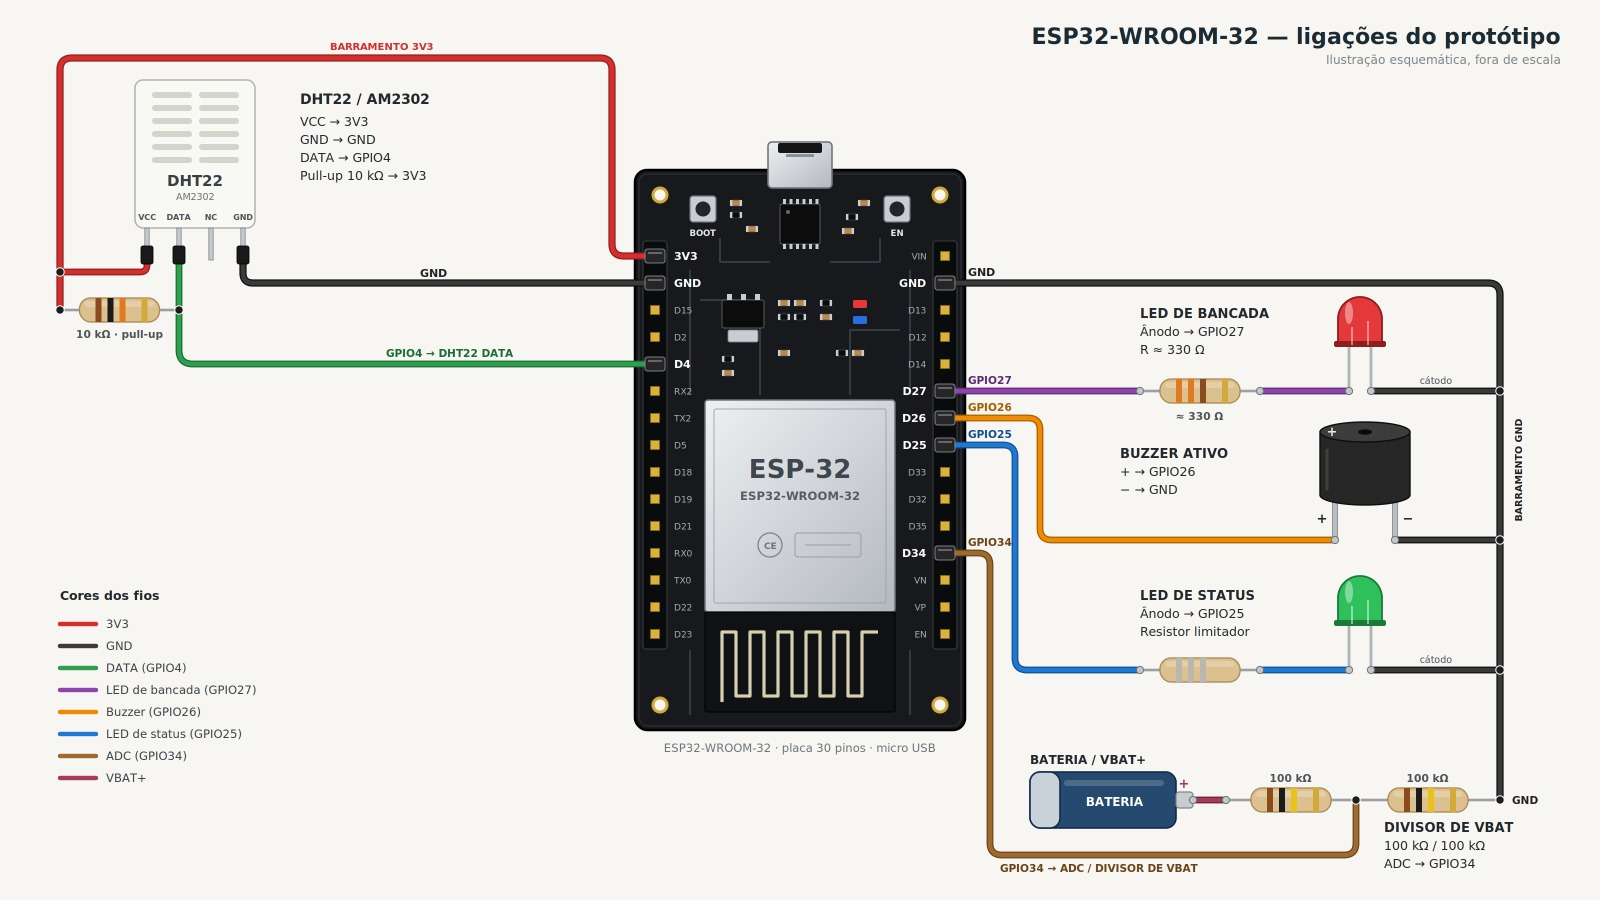
\includegraphics[width=0.9\textwidth]{figuras/mapa-de-barramento.jpeg}
\caption{Ligações do protótipo na placa ESP32}
\label{fig:montagem}
\fonte{Elaborada pela equipe.}
\end{figure}

\section{Estrutura do firmware}
\label{sec:firmware}

\begin{orientacao}
Descreva a máquina de estados do sistema: quais estados existem, o que
dispara cada transição e quanto tempo o sistema passa em cada um. Os
estados daqui têm de ser os mesmos do orçamento de energia
(Apêndice~\ref{ap:energia}) --- se não forem, um dos dois está errado.

Inclua trechos de código apenas quando o trecho \emph{decide} alguma
coisa: o laço de temporização, a histerese, o tratamento de falha de
leitura. Código de inicialização de biblioteca não precisa aparecer;
ele está no repositório.
\end{orientacao}

Como o nó usa \emph{deep sleep} entre leituras (\DP{4}), o
\texttt{loop()} nunca é retomado: a cada despertar o programa recomeça
do \texttt{setup()}, e é dentro dele que mora todo o ciclo. O sistema
tem quatro estados, os mesmos do Apêndice~\ref{ap:energia}:

\begin{description}[style=unboxed, leftmargin=0.6cm]
  \item[\textsc{acorda e configura}] --- inicializa os pinos com buzzer
    e LED de alarme em \texttt{LOW}, carrega a configuração da NVS e
    abre uma janela de \SI{4}{\second} para comandos pela porta serial
    (Seção~\ref{sec:config}). Se nada chegar, segue adiante. Dura
    $\approx$\SI{4}{\second}.
  \item[\textsc{lê}] --- faz 5 amostras do DHT22 espaçadas de
    \SI{2.1}{\second}, calcula a mediana e atualiza a média exponencial
    (Seção~\ref{sec:sinal}). Dura $\approx$\SI{8,4}{\second}.
  \item[\textsc{aciona o atuador}] --- só existe no ciclo em que a
    leitura está fora da faixa: buzzer e LED ficam ligados por
    \SI{3}{\second} e são desligados antes do sono
    (Seção~\ref{sec:decisao}). Nos demais ciclos dura zero.
  \item[\textsc{dorme}] --- \emph{deep sleep} com despertar por
    temporizador. A duração depende do resultado do ciclo:
    \SI{600}{\second} (intervalo normal, \RF{01}) se a leitura estava
    dentro da faixa, ou \SI{60}{\second} (intervalo de alarme) se
    estava fora. Ambos são configuráveis (Seção~\ref{sec:config}).
\end{description}

As transições são todas sequenciais e temporizadas, exceto a que decide
qual intervalo de sono usar, que depende da avaliação de faixa. Os
$\approx$\SI{12}{\second} somados dos três estados acordados são o
\texttt{T\_ACORDADO\_S} do orçamento de energia (\bancada). A
Listagem~\ref{lst:laco} mostra o esqueleto do \texttt{setup()} com as
decisões que importam; a inicialização de bibliotecas e as mensagens de
diagnóstico ficaram no repositório.

\begin{lstlisting}[style=arduino,
  caption={Esqueleto do ciclo: tudo mora no \texttt{setup()}, e o intervalo de sono é decidido no fim},
  label={lst:laco}]
RTC_DATA_ATTR float    emaTemp = NAN, emaHum = NAN;   // atravessam o sono
RTC_DATA_ATTR uint32_t falhasConsecutivas = 0;

void setup() {
  digitalWrite(BUZZER_PIN, LOW);      // estado seguro antes de tudo
  digitalWrite(ALARME_LED_PIN, LOW);
  carregarConfiguracao();             // NVS -> cfg (intervalos e faixa)
  talvezEntrarModoConfig();           // janela de 4 s por comandos SET

  float t, h;
  bool emAlarme = false;
  if (lerDHTFiltrado(t, h)) {         // mediana de 5 amostras
    falhasConsecutivas = 0;
    emaTemp = EMA_ALPHA * t + (1.0f - EMA_ALPHA) * emaTemp;
    emaHum  = EMA_ALPHA * h + (1.0f - EMA_ALPHA) * emaHum;
    emAlarme = avaliarAlarme(t, h);   // usa a mediana, nao a EMA
  } else {
    falhasConsecutivas++;             // declara falha; nao inventa numero
  }

  dormir(emAlarme ? cfg.intervaloAlarmeS : cfg.intervaloNormalS);
}

void loop() { /* nunca executa: deep sleep reinicia no setup() */ }
\end{lstlisting}

O que precisa atravessar o sono está em memória RTC
(\texttt{RTC\_DATA\_ATTR}): contador de despertares, as duas médias
exponenciais e a contagem de falhas consecutivas. Tudo o mais é
recalculado a cada ciclo. A configuração, por sua vez, sobrevive de
outra forma --- pela NVS, que persiste mesmo com o nó desligado.

\subsection{Configuração em tempo de execução}
\label{sec:config}

Na primeira versão, o intervalo de leitura era um \texttt{\#define}.
Isso atende um único cenário, mas a Cap.~\ref{cap:requisitos} exige
que a faixa seja configurável por ambiente (\RF{02}), e o mesmo
argumento vale para o intervalo: uma câmara fria de farmácia e uma sala
de equipamentos não pedem a mesma frequência de checagem, e recompilar
o \emph{firmware} para cada instalação não é solução de produto. Os
seis parâmetros da Tabela~\ref{tab:config} passaram a ser gravados na
NVS pela biblioteca \texttt{Preferences} (inclusa no \emph{core} do
ESP32), sob o \emph{namespace} \texttt{termolog}.

\begin{table}[H]
\centering
\caption{Parâmetros gravados na NVS e seus padrões de fábrica}
\label{tab:config}
\footnotesize
\begin{tabular}{@{}L{4.4cm}L{4.6cm}L{4.4cm}@{}}
\toprule
\textbf{Parâmetro} & \textbf{Comando serial} & \textbf{Padrão de fábrica} \\
\midrule
Intervalo normal entre leituras & \texttt{SET INTERVALO=<s>} & \SI{600}{\second} (\RF{01}) \\
Intervalo enquanto em alarme    & \texttt{SET INTERVALO\_ALARME=<s>} & \SI{60}{\second} \\
Temperatura mínima              & \texttt{SET TEMP\_MIN=<\textdegree C>} & \SI{15}{\celsius} \\
Temperatura máxima              & \texttt{SET TEMP\_MAX=<\textdegree C>} & \SI{25}{\celsius} \\
Umidade relativa mínima         & \texttt{SET UMID\_MIN=<\%>} & 40\,\% UR \\
Umidade relativa máxima         & \texttt{SET UMID\_MAX=<\%>} & 70\,\% UR \\
\bottomrule
\end{tabular}
\fonte{Elaborada pela equipe. Os limiares padrão são os do cenário de validação (farmácia de manipulação, Cap.~\ref{cap:problema}) e devem ser ajustados por ambiente na instalação.}
\end{table}

Os comandos são aceitos pelo monitor serial (\SI{115200}{\baud}) nos
primeiros \SI{4}{\second} após energizar; cada comando aceito é gravado
imediatamente e renova a janela por mais \SI{4}{\second}.
\texttt{SHOW} imprime a configuração em uso e \texttt{RESET} restaura
os padrões. Em campo, sem ninguém na porta serial, a janela expira e o
ciclo segue sozinho com a última configuração gravada.

Duas ressalvas de custo, ambas declaradas para não serem descobertas
depois:

\begin{itemize}
  \item \textbf{O custo da biblioteca em si é desprezível.} A leitura
    da NVS no despertar (\texttt{begin}, seis \texttt{get},
    \texttt{end}) leva alguns milissegundos, invisíveis diante dos
    \SI{8.4}{\second} que o próprio sensor impõe. Escrita só ocorre em
    \texttt{SET}, \texttt{RESET} ou no primeiro boot --- nunca a cada
    ciclo ---, então o desgaste da \emph{flash} não entra na conta.
  \item \textbf{O custo real é a janela serial}, não a biblioteca:
    \SI{4}{\second} de nó acordado a $\approx$\SI{45}{\milli\ampere}
    equivalem a $\approx$\SI{0.05}{\mAh} por ciclo, ou
    $\approx$\SI{7}{\mAh}/dia no intervalo de 10 min --- cerca de
    10\,\% do orçamento diário. Esse tempo já está incluído nos
    \SI{12}{\second} de \texttt{T\_ACORDADO\_S} do
    Apêndice~\ref{ap:energia}; reduzir ou condicionar a janela (por
    exemplo, só abri-la quando a porta serial estiver conectada) é uma
    otimização registrada para o próximo ciclo.
\end{itemize}

Gravar parâmetros na NVS não contradiz a decisão de não guardar
leituras no nó (\DP{7}): o que se guarda é meia
dúzia de números fixos até que alguém os troque, não uma série
temporal.

\section{Lógica de decisão e atuação}
\label{sec:decisao}

\begin{orientacao}
Qual é a regra que liga a leitura ao atuador, e por que ela tem essa
forma. Se há histerese, diga quais são os dois limiares e como foram
escolhidos --- limiar escolhido \enquote{no olho} é resposta aceitável
desde que declarada e acompanhada do que aconteceu quando a equipe
testou. Se não há histerese, explique por que o relé não castanhola.
\end{orientacao}

A regra é uma comparação de faixa sobre a mediana do ciclo: o alarme
dispara se a temperatura estiver abaixo do mínimo ou acima do máximo,
\emph{ou} se a umidade estiver abaixo do mínimo ou acima do máximo
(\RF{02}/\RF{03}). A comparação usa a mediana das 5 amostras, e não a
média exponencial, de propósito: a EMA suaviza justamente o tipo de
desvio que o alarme existe para pegar, e um alarme que reage com atraso
a uma câmara fria aquecendo não cumpre \RNF{02}. A
Listagem~\ref{lst:alarme} mostra a função inteira.

\begin{lstlisting}[style=arduino,
  caption={Avaliação de faixa e acionamento do alarme local (buzzer + LED)},
  label={lst:alarme}]
bool avaliarAlarme(float temperaturaC, float umidadeRH) {
  bool foraDaFaixa = (temperaturaC < cfg.tempMinC) ||
                     (temperaturaC > cfg.tempMaxC) ||
                     (umidadeRH   < cfg.umidMinPct) ||
                     (umidadeRH   > cfg.umidMaxPct);
  if (foraDaFaixa) {
    digitalWrite(BUZZER_PIN, HIGH);     // buzzer ativo: nivel alto = som
    digitalWrite(ALARME_LED_PIN, HIGH);
    delay(ALARME_DURACAO_MS);           // 3 s
    digitalWrite(BUZZER_PIN, LOW);
    digitalWrite(ALARME_LED_PIN, LOW);
    return true;                        // -> dormir no intervalo de alarme
  }
  return false;                         // -> dormir no intervalo normal
}
\end{lstlisting}

O acionamento é um \textbf{pulso de \SI{3}{\second} por ciclo}, não um
som contínuo: o buzzer ativo já oscila sozinho e basta manter o pino em
nível alto, mas manter um GPIO ligado durante o \emph{deep sleep}
exigiria \texttt{gpio\_hold\_en()} sobre um pino RTC, o que esta
revisão não faz. Para que um pulso curto não passe despercebido, o nó
compensa \textbf{acordando mais vezes}: enquanto a última leitura
estiver fora da faixa, o próximo sono dura o intervalo de alarme
(\SI{60}{\second}) em vez do normal (\SI{600}{\second}), e o alarme
volta a soar a cada minuto até a condição ser corrigida. Assim que uma
leitura cai dentro da faixa, o pulso simplesmente não ocorre e o nó
volta ao intervalo normal por conta própria --- é isso que atende
\RF{04}, e em até \SI{1}{\minute} após o retorno, bem dentro do limite
de um ciclo exigido.

\begin{table}[H]
\centering
\caption{Parâmetros da lógica de decisão}
\label{tab:limiares}
\footnotesize
\begin{tabular}{@{}L{4.0cm}C{2.6cm}L{6.8cm}@{}}
\toprule
\textbf{Parâmetro} & \textbf{Valor} & \textbf{Como foi escolhido} \\
\midrule
Faixa de temperatura (liga fora dela) & 15 a \SI{25}{\celsius} & cenário de validação (farmácia); configurável por ambiente \\
Faixa de umidade (liga fora dela) & 40 a 70\,\% UR & idem \\
Histerese entre liga e desliga & nenhuma & ver texto: o atuador não tem estado a castanholar \\
Duração do pulso de alarme & \SI{3}{\second} & \estimativa{} (audível em sala; a ajustar após ensaio) \\
Tempo mínimo entre acionamentos & \SI{60}{\second} & intervalo de alarme; \estimativa{} de compromisso energia/resposta \\
\bottomrule
\end{tabular}
\fonte{Elaborada pela equipe.}
\end{table}

\textbf{Por que não há histerese, e por que isso não castanhola.} Um
relé castanhola quando o sinal oscila em torno de um único limiar e o
atuador tem dois estados persistentes que trocam a cada oscilação.
Aqui o atuador não tem estado persistente: ele é ligado e desligado
dentro do mesmo ciclo, e entre dois ciclos há pelo menos
\SI{60}{\second} de sono. O pior caso de uma leitura oscilando na borda
da faixa é, portanto, um pulso de \SI{3}{\second} a cada minuto ---
exatamente o comportamento de alarme desejado, e não um defeito. A
mediana de 5 amostras também reduz a chance de um único valor de borda
disparar o pulso. Se o ensaio \CT{03} mostrar que a borda incomoda na
prática, a histerese entra como um sétimo parâmetro da NVS sem mudar a
estrutura.

\textbf{Custo declarado da mudança de frequência.} Acordar a cada
minuto custa mais que a cada dez. No pior caso --- nó preso fora da
faixa o dia inteiro --- cada ciclo dura \SI{75}{\second}
(\SI{12}{\second} acordado a \SI{46,5}{\milli\ampere}, \SI{3}{\second} de
alarme com mais \SI{35}{\milli\ampere} e \SI{60}{\second} dormindo a
\SI{2}{\milli\ampere}) e consome $\approx$\SI{0,26}{\mAh}; com
\num{1152} ciclos por dia, são $\approx$\SI{295}{\mAh}/dia, contra os \SI{69}{\mAh}/dia
do regime normal. Com a 18650 de \SI{2600}{\mAh} do
Apêndice~\ref{ap:energia}, a autonomia cai de $\approx$30 para
$\approx$7 dias \emph{enquanto o alarme persistir}. A equipe aceita
esse custo porque, por definição, ele só ocorre enquanto algo está
errado --- e sete dias de alarme sem ninguém agir é um problema
operacional, não de bateria. O número usa a corrente de alarme ainda
\estimativa{}; será revisto após a medição em bancada.

\section{Tratamento do sinal}
\label{sec:sinal}

\begin{orientacao}
O que foi feito entre o valor bruto do ADC e o número usado na decisão:
calibração (com a curva e o procedimento), média móvel, descarte de
\emph{outliers}, saturação. Traga o antes e o depois --- um gráfico com
o sinal cru e o sinal tratado vale mais que dois parágrafos. Reaproveite
a análise de ruído de 26/08.
\end{orientacao}

\subsection{Formato de captação do DHT22}

O DHT22 inverte o problema tratado na Aula~05: não há ADC da equipe nem
contagem bruta. O sensor traz o conversor embutido e entrega, por um
protocolo proprietário de um fio, dois números já calibrados de
fábrica --- temperatura em \si{\celsius} com resolução de
\SI{0.1}{\celsius} e umidade relativa em \% UR com resolução de
0,1\,\% --- protegidos por um \emph{checksum} de um byte. A biblioteca
\texttt{DHT} (Adafruit) decodifica o quadro de 40 bits e devolve
\texttt{NaN} quando o \emph{checksum} falha ou o \emph{timing} da
resposta sai da tolerância. Duas consequências fixam o formato de
captação:

\begin{itemize}
  \item \textbf{o erro sistemático não é corrigível por software}: a
    incerteza declarada em \folhadedados{} ($\pm$\SI{0.5}{\celsius};
    $\pm 2$\,\% UR, chegando a $\pm 5$\,\% nas extremidades) é
    impressa junto de cada leitura, para não se perder entre o sensor
    e quem consome o dado (\RNF{04});
  \item \textbf{o sensor impõe um intervalo mínimo de \SI{2}{\second}
    entre leituras}; o \emph{firmware} usa \SI{2.1}{\second}, o que
    limita a 5 o número de amostras que cabem em um ciclo sem
    estourar o tempo acordado orçado.
\end{itemize}

O ruído que resta é de \emph{comunicação}, não de sinal: um bit mal
decodificado por interferência no fio ou por variação de \emph{timing}
produz \texttt{NaN} ou, mais raramente, um valor absurdo isolado --- e
é este o caso de \RNF{05}, quando o compressor da câmara fria liga. A
captação, portanto, é feita em dois estágios com preço declarado:

\begin{enumerate}
  \item \textbf{Mediana de 5 amostras por ciclo.} Cada amostra é uma
    leitura de temperatura e uma de umidade; amostras \texttt{NaN} são
    descartadas na hora. Se menos de 3 das 5 forem válidas, o ciclo é
    declarado como \textbf{falha} --- sem inventar uma mediana a
    partir de dois pontos (Listagem~\ref{lst:leitura}). A mediana
    descarta um \emph{outlier} isolado sem arrastar o resultado, como
    faria uma média aritmética. Custo: $\approx$\SI{8.4}{\second} de
    nó acordado por ciclo.
  \item \textbf{Média exponencial (EMA) entre ciclos}, com
    $\alpha = 0{,}30$, guardada em memória RTC:
    $\text{ema}_{n} = \alpha\,x_n + (1-\alpha)\,\text{ema}_{n-1}$.
    Suaviza a variação natural entre um despertar e o seguinte sem
    exigir histórico nem herdar o atraso de uma janela longa. Custo:
    dois \texttt{float} em RTC; latência de $\approx$3 ciclos para
    acompanhar um degrau. Por isso a EMA é apenas o valor
    \emph{reportado}, e nunca o valor usado na decisão de alarme
    (Seção~\ref{sec:decisao}).
\end{enumerate}

\begin{lstlisting}[style=arduino,
  caption={Captação do DHT22: 5 amostras, descarte de \texttt{NaN}, maioria obrigatória, mediana},
  label={lst:leitura}]
bool lerDHTFiltrado(float &temperaturaC, float &umidadeRH) {
  float amostrasTemp[N_AMOSTRAS], amostrasHum[N_AMOSTRAS];
  int validas = 0;
  for (int i = 0; i < N_AMOSTRAS; i++) {
    float t = dht.readTemperature();
    float h = dht.readHumidity();
    if (!isnan(t) && !isnan(h)) {     // checksum ou timing ruim -> NaN
      amostrasTemp[validas] = t;
      amostrasHum[validas]  = h;
      validas++;
    }
    if (i < N_AMOSTRAS - 1) delay(DHT_MIN_INTERVAL_MS);  // 2100 ms
  }
  if (validas < (N_AMOSTRAS / 2 + 1)) return false;      // < 3 de 5
  temperaturaC = mediana(amostrasTemp, validas);
  umidadeRH    = mediana(amostrasHum, validas);
  return true;
}
\end{lstlisting}

No nó da AP1, o dado sai apenas pela porta serial, no formato da
Listagem~\ref{lst:serial}: mediana e EMA lado a lado, seguidas da
incerteza declarada e, quando há bateria, da tensão lida. O
\emph{firmware} de comunicação da campanha publica, em vez disso, a
leitura única no contrato da Seção~\ref{sec:contrato-dados}; publicar a
mediana é parte da união das duas versões.

\begin{lstlisting}[style=terminal,
  caption={Saída serial de um ciclo com leitura válida},
  label={lst:serial}]
---- Leitura ----
Temperatura (mediana da amostra): 23.40 C
Umidade     (mediana da amostra): 58.10 %RH
Temperatura (media exponencial):  23.12 C
Umidade     (media exponencial):  57.65 %RH
Incerteza declarada (datasheet DHT22): +-0.5 C / +-2 a 5% RH
Tensao da bateria: 3.98 V
Dormindo por 600 segundos...
\end{lstlisting}

O gráfico que mostraria o efeito do filtro, com as amostras brutas e as
medianas lado a lado, ainda não existe: ele depende de um
ensaio dedicado ao \RNF{05}, com o sensor junto a um compressor ligado,
ainda não feito, que produzirá as séries de amostras brutas e de medianas a serem
comparadas. Até lá, o que a equipe pode declarar é o procedimento e o
seu preço, não o efeito medido.

\section{Comportamento em falha}
\label{sec:falha}

\begin{orientacao}
Esta seção é curta e é a que mais separa protótipo de demonstração.
Responda quatro perguntas: o que acontece se o sensor devolver lixo; o
que acontece se a alimentação cair no meio de um acionamento; em que
posição o atuador fica quando o sistema desliga ou dorme; e como alguém
descobre que o sistema parou.
\end{orientacao}

\begin{description}[style=unboxed, leftmargin=0pt, font=\normalfont\bfseries]
  \item[Se o sensor devolver lixo.]\hfill\\
    Amostras com \emph{checksum} inválido viram \texttt{NaN} e são
    descartadas; um valor absurdo isolado é absorvido pela mediana. Se
    menos de 3 das 5 amostras forem válidas, o ciclo é declarado como
    falha: a EMA não é atualizada, \texttt{falhasConsecutivas} é
    incrementada em memória RTC, a causa provável é impressa na
    serial e o nó dorme no intervalo normal. \textbf{Limitação
    declarada:} nesta revisão, um ciclo em falha \emph{não} aciona o
    alarme --- um sensor desconectado é silencioso, e o contador de
    falhas consecutivas é registrado mas ainda não tem consequência.
    Tratar $N$ falhas seguidas como condição de alarme é a mudança
    prevista para o próximo ciclo.
  \item[Se a alimentação cair no meio de um acionamento.]\hfill\\
    O buzzer e o LED apagam com a placa. Ao retornar a energia, a
    primeira ação do \texttt{setup()} é escrever \texttt{LOW} nos dois
    pinos, antes de qualquer leitura; a configuração é recarregada da
    NVS intacta (a gravação só ocorre em comandos \texttt{SET}, nunca
    durante o ciclo). O que se perde é a memória RTC --- EMA, contador
    de despertares e de falhas ---, que reinicia como no primeiro
    boot; a EMA é então semeada com a primeira mediana válida.
  \item[Em que posição o atuador fica quando o nó desliga ou dorme.]\hfill\\
    Desligado. O alarme é sempre desligado explicitamente antes de
    \texttt{esp\_deep\_sleep\_start()}, e o \emph{deep sleep} não
    retém o nível dos GPIO (não há \texttt{gpio\_hold\_en()}). Não
    existe estado em que o buzzer fique ligado sem o processador
    acordado; o estado seguro é o silêncio.
  \item[Como alguém descobre que o sistema parou.]\hfill\\
    No nó da AP1, não descobre --- e isso é dito com todas as letras.
    O LED de status acende apenas enquanto o nó está acordado
    ($\approx$\SI{12}{\second} a cada 10 min), o que serve à bancada
    mas não a um operador; sem rede, um nó com bateria esgotada ou
    sensor solto simplesmente deixa de acordar (ou de alarmar) sem
    avisar ninguém. Um \emph{watchdog} externo ou um
    \emph{heartbeat} pela rede é o que resolve, e é o que o
    \emph{firmware} de comunicação trouxe.

    \textbf{Na AP2:} com a rede, o nó deixa com o \emph{broker}, ao
    conectar, a mensagem \texttt{offline} retida no tópico
    \texttt{status}. Se ele morrer sem avisar, o \emph{broker} a publica
    em nome dele depois de $1{,}5 \times$ o \emph{keepalive} de
    \SI{30}{\second}, ou seja, cerca de \SI{45}{\second} depois da última
    mensagem do nó (\RF{07}; no \CT{10}, \SI{46}{\second}). Quem olha esse
    tópico é o gravador, que o grava no CSV, e quem abrir o MQTT Explorer;
    ninguém recebe um aviso automático. Na campanha, as quedas foram vistas
    no terminal do gravador por quem acompanhava a coleta, e contadas
    depois no CSV.
  \item[Se a rede ou o \emph{broker} caírem (AP2).]\hfill\\
    No nó da AP1, a decisão de alarme não passa pela rede (\DP{5}): ela
    usa a faixa gravada na NVS e continuaria funcionando sem WiFi e sem
    \emph{broker}. O que se perde é o registro. No \emph{firmware} da
    campanha, a leitura só é feita e publicada quando há conexão com o
    \emph{broker}, e não há fila local: sem conexão, a leitura daquele
    período simplesmente não existe, e o \texttt{seq} não avança. O
    buraco não aparece como salto de \texttt{seq} no \texttt{qualidade.py},
    só na completude. Na queda de WiFi de \SI{101}{\second} do \CT{09},
    cerca de 19 leituras se perderam assim.
\end{description}

\section{Firmware de comunicação}
\label{sec:firmware-com}

\begin{orientacao}
Novo na AP2. Os estados da conexão (desligado, conectando, conectado), a
reconexão, a fila local, o NTP e o testamento. Inclua só os trechos de
código que decidem algo --- o laço que não pode ficar parado mais que
1,5 $\times$ \emph{keepalive}, a montagem do JSON com \texttt{boot} e
\texttt{seq}, o que fazer com a leitura quando não há \emph{broker}. Se
a equipe alterou o gravador, diga o quê, aqui. A versão descrita é a que
rodou na campanha, no \emph{commit} da Seção~\ref{sec:repositorio}.
\end{orientacao}

Esta seção descreve o \emph{firmware} que rodou nos testes de falha e
na campanha de 24/10: \texttt{sketch/sketch.ino}, gravado no
\emph{commit} \texttt{7b4482e} da branch \texttt{lab3} (na pasta
\texttt{wokwi/}) e entregue, sem mudança de código, na pasta
\texttt{firmware/} do \emph{commit} da entrega
(Seção~\ref{sec:repositorio}). É o mesmo arquivo no Wokwi e na placa;
na placa, ele é compilado e gravado pelo PlatformIO
(\texttt{platformio.ini}).

\subsection{Estados da conexão}

O laço tem três estados, testados nesta ordem a cada volta:
\textsc{sem rede} (o WiFi não está associado: o laço retorna sem fazer
nada, e o \emph{core} do ESP32 reassocia sozinho), \textsc{sem
\emph{broker}} (há rede, mas a conexão MQTT caiu: uma nova tentativa a
cada \SI{5}{\second}) e \textsc{conectado} (\texttt{mqtt.loop()} entrega o
que chegou e mantém a conexão viva, e uma leitura é publicada a cada
\texttt{periodo\_s}, \SI{5}{\second} por padrão). Não há \emph{deep
sleep} neste \emph{firmware} (\DP{6}): o período de leitura é contado com
\texttt{millis()}, sem \texttt{delay()}, e a leitura do DHT22 é uma só
por período. Quando a leitura falha, o nó publica o \texttt{rssi\_dbm}
no lugar das grandezas, e o \texttt{seq} avança do mesmo jeito.

\begin{lstlisting}[style=terminal,
  caption={O laço do \emph{firmware} da campanha (\texttt{sketch.ino}, \emph{commit} \texttt{7b4482e})},
  label={lst:laco-com}]
if (WiFi.status() != WL_CONNECTED) { avisouWiFi = false; return; }  // SEM REDE
if (!mqtt.connected() && millis() - ultimaTentativa > 5000) {     // SEM BROKER
  ultimaTentativa = millis(); conectaBroker();
}
mqtt.loop();                                   // mantem a conexao viva
if (mqtt.connected() && millis() - ultimaLeitura >= periodo_s * 1000UL) {
  ultimaLeitura = millis(); publicaTelemetria();   // CONECTADO: le e publica
}
\end{lstlisting}

As duas condições de \texttt{mqtt.connected()} são a decisão que mais
pesou na campanha: sem \emph{broker}, nada é lido. E o \texttt{seq} é
incrementado dentro de \texttt{publicaTelemetria()}, antes de publicar;
por isso só uma publicação tentada e perdida abre buraco no \texttt{seq}
(foram 2 na campanha).

Quando a leitura filtrada da AP1 for trazida para este laço, as 5
amostras do DHT22 espaçadas de \SI{2,1}{\second} e o pulso de alarme de
\SI{3}{\second} vão somar cerca de \SI{11,4}{\second} sem chamar
\texttt{mqtt.loop()}. Isso cabe nos \SI{45}{\second} ($1{,}5 \times$
\emph{keepalive}) que o \emph{broker} espera antes de dar o nó por morto,
mas impede reduzir o \emph{keepalive} abaixo de cerca de
\SI{8}{\second}.

\subsection{Reconexão e fila local}

O WiFi reconecta sozinho, e o \emph{broker} é tentado a cada
\SI{5}{\second} enquanto houver rede. Como a sessão é persistente
(\texttt{setCleanSession(false)}) e o \emph{client ID} é fixo
(\texttt{ufpi-iot26-eq01-no02}), ao voltar o nó recebe as mensagens
de configuração que o \emph{broker} guardou para ele. \textbf{Não há
fila local}: a leitura que não pôde ser publicada nunca chega a ser
feita. A biblioteca MQTT espera no máximo \SI{1}{\second} pela resposta
do \emph{broker} a cada operação e derruba a conexão quando o tempo
estoura; é a causa provável da fase degradada da campanha
(Seção~\ref{sec:qualidade}), ainda não confirmada.

\subsection{Hora da leitura (NTP)}

O relógio é acertado por \texttt{configTime()} com os servidores
\texttt{pool.ntp.org} e \texttt{time.google.com}, chamado logo depois de
pedir a associação ao WiFi. O campo \texttt{ts} leva o instante da
\emph{medição} em segundos desde 1970 (UTC); enquanto o relógio do nó
ainda marcar uma data anterior a novembro de 2023 (\texttt{time()} $<$
\texttt{1700000000}), o \texttt{ts} sai como \texttt{null}, em vez de uma
hora errada. Na medição de 23/10, o relógio acertou cerca de
\SI{2}{\second} depois do pedido (log da sessão
\texttt{2026-10-23\_172639}). Nos três reinícios de 24/10, o NTP acertou
antes da primeira publicação, e nenhuma leitura saiu com \texttt{ts}
nulo (\CT{13}). Se sair, a leitura é mantida e contada: o
\texttt{qualidade.py} a posiciona pela hora de chegada ao gravador.

A Listagem~\ref{lst:publica} é a montagem do JSON, que decide três
coisas: o \texttt{seq} avança antes de publicar (por isso só uma
publicação tentada e perdida abre buraco nele), o \texttt{ts} vira
\texttt{null} antes do NTP, e a leitura que falha manda o
\texttt{rssi\_dbm} no lugar das grandezas, em vez de um número
inventado. Não há \texttt{boot}: é a lacuna do \RF{08}.

\begin{lstlisting}[style=arduino,
  caption={Montagem e publicação da leitura (\texttt{sketch.ino}, \emph{commit} \texttt{7b4482e}; trecho sem alteração)},
  label={lst:publica}]
void publicaTelemetria() {
  JsonDocument doc;
  doc["id"]  = idNo;                      // "eq01-no02"
  doc["seq"] = ++seq;
  if (time(nullptr) > 1700000000) doc["ts"] = (uint32_t)time(nullptr);
  else                            doc["ts"] = nullptr;   // antes do NTP
  leSensores(doc);        // temp_c e umid_pct, ou rssi_dbm se o DHT22 falhar
  char buf[256];
  serializeJson(doc, buf, sizeof(buf));
  bool ok = mqtt.publish(tTele, buf, false, 1);   // nao retido, QoS 1
  Serial.printf("[pub] %s  %s  %s\n", tTele, buf, ok ? "" : "<- FALHOU");
}
\end{lstlisting}

\subsection{\emph{Status} e testamento}

Ao conectar, o nó registra no \emph{broker} o testamento
\texttt{offline} (QoS~1, retido) no tópico \texttt{status} e, em seguida,
publica ele mesmo \texttt{online}, também retido, para que quem chegar
depois veja o estado atual sem esperar a próxima leitura. O
\emph{keepalive} é de \SI{30}{\second}: sem notícias do nó por
\SI{45}{\second}, o \emph{broker} publica o \texttt{offline} em nome
dele. A conexão é cifrada (TLS, porta 8883), mas o nó usa
\texttt{setInsecure()}, isto é, não confere o certificado do servidor;
é o atalho de sala do Lab~03, declarado como limitação
(Cap.~\ref{cap:conclusao}). A Listagem~\ref{lst:conecta} mostra a
ordem que importa: testamento, sessão persistente e \emph{keepalive}
são configurados \emph{antes} do \texttt{connect()}, porque vão no
pacote CONNECT; o \texttt{online} e a assinatura do \texttt{config} só
depois de conectado.

\begin{lstlisting}[style=arduino,
  caption={Conexão ao \emph{broker}: testamento, sessão persistente e \emph{keepalive} (\texttt{sketch.ino}, \emph{commit} \texttt{7b4482e}; mensagens de diagnóstico omitidas)},
  label={lst:conecta}]
void conectaBroker() {
  mqtt.setWill(tStatus, "offline", true, 1);  // retido, QoS 1
  mqtt.setCleanSession(false);                // sessao persistente
  mqtt.setKeepAlive(30);                      // morto apos ~45 s sem noticias
  if (!mqtt.connect(clientId, MQTT_USUARIO, MQTT_SENHA)) return;  // tenta de novo em 5 s
  mqtt.publish(tStatus, "online", true, 1);   // retido: quem chega depois ve
  mqtt.subscribe(tConfig, 1);                 // canal de volta (periodo_s)
}
\end{lstlisting}

\subsection{Gravador}

O gravador é o \texttt{gravador.py} do Lab~03 (pasta
\texttt{gravador/}, mesmo \emph{commit}), um assinante MQTT em Python
(\texttt{paho-mqtt}) que rodou no notebook de João Pedro Saleh, ligado
na tomada, com o comando
\texttt{python gravador.py -{}-host broker.hivemq.com -{}-equipe eq01}.
Ele assina \texttt{ufpi-iot26/eq01/+/telemetria} e \texttt{ufpi-iot26/eq01/+/status}
com QoS~1, com \emph{client ID} fixo (\texttt{ufpi-iot26-eq01-gravador}),
sessão persistente e TLS verificado pelas autoridades certificadoras do
sistema (sem \texttt{-{}-usuario}, ele não usa o \texttt{ca\_raiz.pem} do
\emph{broker} da turma), e grava cada mensagem em
\texttt{dados/mensagens.csv} com as colunas \texttt{t\_chegada},
\texttt{chegada}, \texttt{topico}, \texttt{retido} e \texttt{payload},
com \emph{flush} a cada linha. Ele não descarta repetidas: grava tudo o
que chega, e a deduplicação fica para o \texttt{qualidade.py}.

\textbf{O que a equipe mudou nos \emph{scripts} do docente}
(comparação com a versão distribuída no Lab~03):

\begin{itemize}
  \item \texttt{gravador.py}: o \texttt{-{}-usuario} deixou de ser
    obrigatório. Sem ele, o gravador conecta sem login ao \emph{broker}
    público, assina a árvore dada em \texttt{-{}-equipe}, monta o
    \emph{client ID} com o nome da equipe e confere o certificado do
    servidor pelas autoridades do sistema, em vez do
    \texttt{ca\_raiz.pem}. Com \texttt{-{}-usuario}, o comportamento é o
    original. A gravação, as colunas, o QoS e a sessão não mudaram.
  \item \texttt{qualidade.py}: ganhou a opção \texttt{-{}-periodo}
    (padrão \SI{5}{\second}) e três saídas novas, calculadas pela hora
    da medição (\texttt{ts}, ou a de chegada se ele for nulo): as
    leituras esperadas, $(\text{fim} - \text{início}) \div
    \text{período} + 1$, na janela \texttt{-{}-de}/\texttt{-{}-ate} ou da
    primeira à última leitura; a completude, leituras únicas $\div$
    esperadas; e as lacunas maiores que $1{,}5 \times$ o período, com as
    dez maiores listadas. A versão do docente não calculava nenhuma das
    três, e o \texttt{seq} sozinho não mostra a leitura que nunca foi
    feita. A contagem de faltas, repetidas e reinícios e o filtro de
    horário ficaram como estavam.
  \item \texttt{grafico.py}: novo. Desenha a série pela hora da
    medição, corta a linha onde falta leitura, sem interpolar, e mostra
    os \texttt{offline} a cada \SI{10}{\minute}
    (Figura~\ref{fig:resultado}).
\end{itemize}

\noindent Nenhum dos três usa o \texttt{boot}, que o contrato da
campanha não tem.

\subsection{Ponte para o servidor do produto}
\label{sec:ponte}

O servidor do produto recebe leituras em lotes, de um nó central
autenticado por chave de API (\texttt{POST /gateways/\{id\}/leituras}).
Como o nó central ainda não existe em hardware, a equipe escreveu o papel
dele como uma ponte em Python, \texttt{integracao/ponte\_api.py}, que lê
o CSV bruto do gravador e entrega as leituras ao servidor no contrato
dele. A Tabela~\ref{tab:ponte} mostra a conversão; o teste está no
\CT{16}.

\begin{table}[H]
\centering
\caption{Do contrato da campanha ao contrato da API do produto}
\label{tab:ponte}
\footnotesize
\begin{tabular}{@{}L{3.4cm}L{3.6cm}L{6.6cm}@{}}
\toprule
\textbf{Campanha (MQTT)} & \textbf{API do produto} & \textbf{Conversão} \\
\midrule
\texttt{id} (\texttt{eq01-no02}) & \texttt{sensor\_id} & o sensor cadastrado na sala, ligado ao nó central que envia \\
\texttt{temp\_c}, \texttt{umid\_pct} & \texttt{temperatura}, \texttt{umidade} & número real; leituras só com \texttt{rssi\_dbm} ficam de fora \\
\texttt{ts} (época Unix, NTP) & \texttt{data\_hora} & ISO~8601 com fuso UTC: a hora continua sendo a da medição, carimbada no nó \\
\texttt{seq} e reinícios & \texttt{lote\_id} & UUID5 do nó e do intervalo de \texttt{seq} do lote: reenviar o mesmo lote não grava nada de novo \\
--- & \texttt{versao\_config} & 0 (o nó da campanha não tem configuração remota no servidor) \\
\bottomrule
\end{tabular}
\fonte{Elaborada pela equipe, a partir de \texttt{integracao/ponte\_api.py} e dos esquemas da API (\texttt{leituras/schemas.py}).}
\end{table}

Os lotes têm até 100 leituras, o máximo que a API aceita, e as repetidas
saem pela mesma regra do \texttt{qualidade.py} (\texttt{seq} repetido
dentro do trecho entre reinícios). A ponte só usa a biblioteca padrão do
Python.

\subsection{O ciclo do nó que dorme, em HTTP}
\label{sec:firmware-http}
O \emph{firmware} da campanha fica sempre conectado (\DP{6}, opção b).
O ciclo que um nó em \emph{deep sleep} pagaria a cada despertar (opção a)
também foi implementado e rodou na placa: é o \emph{firmware} da
ferramenta da Aula~10 (branch \texttt{apendice\_b}, \emph{commit}
\texttt{f30a6de}, pasta \texttt{firmware/}), o mesmo que mediu a linha
do rádio da Seção~\ref{sec:custo-radio}. A cada ciclo ele liga o rádio,
associa ao roteador, obtém o IP, resolve o nome do servidor, conecta,
publica a leitura por HTTP (ou HTTPS) e desliga o rádio, cronometrando
cada fase com \texttt{millis()}. Três decisões dele valem para o produto:

\begin{itemize}
  \item o \texttt{seq} fica em \texttt{RTC\_DATA\_ATTR}, a memória que
    atravessa o \emph{deep sleep} (Aula~08), para que um nó que dorme
    entre leituras não recomece a contagem a cada despertar;
  \item a leitura leva o contrato da versão~1 (Listagem~\ref{lst:payload}):
    \texttt{ts} \texttt{null} antes do NTP e \texttt{temp\_c} e
    \texttt{umid\_pct} \texttt{null} quando o DHT22 falha, em vez de um
    número inventado;
  \item o envio passa por \texttt{postComPolitica()}, que separa o erro
    do nó (4xx: não repete) do erro do caminho (5xx ou sem rede: repete
    com espera de \SI{1}{\second} e depois \SI{2}{\second}, até três
    tentativas). O ensaio dessa política é o \CT{17}.
\end{itemize}

Na sessão de 23/10, esse \emph{firmware} entregou 35 leituras
confirmadas com resposta 2xx, sem duplicata, e o gravador apontou as
três lacunas de \texttt{seq}: os 2 envios que ficaram sem resposta 2xx e
o corpo inválido do \CT{17} (\texttt{gravador/dados/resumo.md}). Ele não tem \emph{deep sleep} de
fato, nem MQTT, nem fila local: cada ciclo é disparado por uma tecla, e
o nó volta ao laço em vez de dormir. O que ele prova é o pedaço mais caro
da opção (a), o ciclo de rádio inteiro, com os tempos da
Tabela~\ref{tab:custo-radio}.

\subsection{ESP-NOW e BLE em bancada, no lugar do LoRa}
\label{sec:espnow-bancada}
Na arquitetura proposta para o produto (Figura~\ref{fig:arquitetura}),
o nó de borda manda a leitura por LoRa a um nó central. Como o módulo
LoRa comprado pela equipe não chegou a tempo, a equipe montou esse salto
com os dois rádios que o ESP32 já tem, para avaliar se algum deles
poderia substituir o LoRa. As baterias de alcance de 24/10
(Seção~\ref{sec:tecnologia}) usaram o dado do projeto, e não um pacote
sintético: o sensor
(branch \texttt{teste-esp-now}, \texttt{firmware/sensor/}) é um ESP32
com o DHT22 no GPIO4, o mesmo pino da AP1, e o \emph{gateway}
(\texttt{firmware/gateway/}) é um segundo ESP32 no papel do nó central.
A versão BLE (branch \texttt{teste-ble}) usa o mesmo pacote. O que o
\emph{firmware} de ESP-NOW faz:

\begin{itemize}
  \item o sensor lê o DHT22 a cada \SI{2,1}{\second} e põe a última
    leitura (\texttt{temp\_c\_x10} e \texttt{umid\_pct\_x10}) em cada
    pacote de 25 bytes da Tabela~\ref{tab:gatt}; leitura inválida vai com
    um valor-sentinela, e não com um número inventado;
  \item o sensor começa em \emph{broadcast}, aprende o endereço do
    \emph{gateway} no primeiro ACK e passa a \emph{unicast}, com
    confirmação e retransmissão da camada MAC; os envios que falham
    entram no contador \texttt{tx\_falhas}, que viaja no pacote;
  \item o \emph{gateway} tira o pacote do \emph{callback} do rádio por
    uma fila, devolve o ACK ao sensor e imprime uma linha por pacote,
    com as grandezas e o número de pacotes descartados por fila cheia.
\end{itemize}

Até \SI{8}{\metre} com uma parede, chegaram ao \emph{gateway} os
\num{3010} pacotes enviados, sem perda; das \num{3010} linhas gravadas,
só uma veio com a temperatura inválida, a \SI{5}{\metre}
(\texttt{testes\_24-10-26/brutos/}, \emph{commit} \texttt{affb704}).
Como a leitura só se renova a cada \SI{2,1}{\second} e o pacote sai a
cada \SI{100}{\milli\second}, a mesma leitura se repete em cerca de 20
pacotes seguidos: é uma taxa de teste de enlace, e não de operação.

O ESP-NOW funcionou bem de perto: entregou todos os pacotes até
\SI{8}{\metre} com uma parede. Mais longe, perdeu 18,7\,\% a
\SI{11}{\metre} com duas paredes e 97,6\,\% a \SI{18}{\metre}; o BLE,
nas mesmas posições, chegou cerca de \SI{8,7}{\deci\bel} mais fraco,
entregou só 40\,\% a \SI{11}{\metre} e não fez enlace a \SI{13}{\metre}
(Tabela~\ref{tab:mudancas}, \CT{15}). O resultado do ESP-NOW vale para
o ambiente do teste, uma casa com paredes de alvenaria e portas de
madeira, e pode não se repetir no nosso caso de uso: na farmácia, o nó
de borda pode ficar dentro de um freezer ou de uma câmara fria, de
paredes metálicas, que não foram testadas com nenhum rádio, a uma
distância do nó central que ainda não se conhece
(Seção~\ref{sec:local}). Por isso o produto mantém o LoRa (\DP{8}),
que em \SI{915}{\mega\hertz} deve atravessar melhor esses obstáculos, e
o enlace LoRa será montado quando o módulo chegar. O ESP-NOW continua
como alternativa para os nós que ficarem na mesma sala do nó central. O trecho seguinte, do nó central ao
servidor, foi exercitado à parte pela ponte da Seção~\ref{sec:ponte}
(\CT{16}).

\section{Repositório}
\label{sec:repositorio}

\begin{orientacao}
Link do repositório da equipe, com a estrutura de pastas e o
\emph{commit} exato que corresponde a este relatório. Entrega sem
\emph{commit} identificado obriga o docente a adivinhar qual versão
avaliar, e a adivinhação nunca favorece a equipe.
\end{orientacao}

\noindent Repositório: \url{\repositorioEquipe}\\
\emph{Commit} da entrega: o marcado com a \emph{tag} \texttt{ap2} na
branch \texttt{entrega-ap2} (\texttt{git checkout ap2}). Ele parte do
\emph{commit} \texttt{7b4482e} da branch \texttt{lab3} (24/10/2026, o
que rodou nos testes e na campanha), com o \emph{firmware}, o gravador e
os dados, e acrescenta a integração com o servidor do produto, em
\texttt{integracao/}, e as fontes deste relatório, em \texttt{docs/}.
Os arquivos de dados são os mesmos do \texttt{7b4482e}; nos dois
\texttt{.md} de \texttt{dados/}, só o caminho do \emph{firmware} e o
pino do DHT22 foram corrigidos. Como o PDF é gerado a partir de \texttt{docs/}, ele
não pode citar o próprio \emph{hash}; a \emph{tag} identifica a versão
sem ambiguidade, e \texttt{git rev-parse ap2} devolve o \emph{hash}.

\medskip
\noindent As medições citadas neste relatório estão em branches de
trabalho do mesmo repositório, cada uma com o próprio README e os dados
brutos:

\begin{itemize}
  \item \texttt{apendice\_b} (\emph{commit} \texttt{f30a6de}, 23/10):
    ferramenta da Aula~10 que cronometra o ciclo
    conectar--publicar--desconectar e gera a linha do rádio do
    Apêndice~\ref{ap:energia} (Seção~\ref{sec:custo-radio});
  \item \texttt{teste-esp-now} (\texttt{affb704}, 24/10) e
    \texttt{teste-ble} (\texttt{f149308}, 24/10): baterias de alcance e
    desempenho dos dois rádios nas mesmas posições
    (Seção~\ref{sec:tecnologia});
  \item \texttt{lab3} (\texttt{7b4482e}, 24/10): \emph{firmware} MQTT,
    gravador e os dados dos testes de falha e da campanha
    (Seções~\ref{sec:firmware-com}, \ref{sec:campanha}
    e~\ref{sec:testes-ap2}).
\end{itemize}

\medskip
\noindent Estrutura do \emph{commit} da entrega (\emph{tag} \texttt{ap2}):

\begin{lstlisting}[style=terminal]
firmware/sketch/sketch.ino          firmware do no (o mesmo no Wokwi e na placa)
firmware/sketch/secrets.example.h   modelo de credenciais; secrets.h no .gitignore
firmware/platformio.ini             compila e grava o sketch na placa
firmware/diagram.json               circuito do Wokwi
gravador/gravador.py             assina os topicos e grava dados/mensagens.csv
gravador/qualidade.py            completude, lacunas, faltas e repetidas
gravador/grafico.py              serie temporal com as lacunas a mostra
dados/testes_falha_24-10-26/     CSV bruto, saida do qualidade.py, eventos
dados/campanha_24-10-26/         CSV bruto, saida do qualidade.py, grafico
integracao/ponte_api.py          leva o CSV ao servidor do produto, em lotes
integracao/resultado_25-10-26.md teste da ponte contra a API (CT-16)
integracao/conta_reconexoes.py   tempo de reconexao contado no CSV (CT-09)
docs/                            fontes LaTeX deste relatorio e figuras
README.md                        metodologia e passo a passo
\end{lstlisting}

\noindent Na \texttt{lab3}, a pasta do \emph{firmware} se chamava
\texttt{wokwi/}; no \emph{commit} da entrega ela foi renomeada para
\texttt{firmware/}, como pedem as instruções da AP2, sem mudança no
conteúdo. O \emph{firmware} da AP1 (\texttt{esp32\_dht22.ino}) continua
na branch \texttt{victor\#sensores}.

\noindent Dependências do \emph{firmware} da campanha, declaradas no
\texttt{platformio.ini}: plataforma \texttt{espressif32@8.0.0}, placa
\texttt{esp32dev}, \texttt{256dpi/MQTT@\^{}2.5.2},
\texttt{bblanchon/ArduinoJson@\^{}7.2.1} e
\texttt{beegee-tokyo/DHT sensor library for ESPx@\^{}1.19}. O monitor
serial abre em \SI{115200}{\baud}. Para gravar: \texttt{pio run -t
upload} na pasta \texttt{firmware/}, com o \texttt{secrets.h} preenchido a
partir do \texttt{secrets.example.h}. O \texttt{diagram.json} do Wokwi
liga o DHT22 ao \texttt{GPIO15}, e o \texttt{sketch.ino} lê o
\texttt{GPIO4}, que é o pino da placa; no Wokwi, como está, o DHT22 não
seria lido. O \emph{firmware} da AP1 usa as bibliotecas \texttt{DHT
sensor library} e \texttt{Adafruit Unified Sensor}, e o
\texttt{Preferences} do \emph{core} do ESP32; grava-se com a placa
\texttt{WEMOS D1 R32} selecionada na Arduino IDE.
